\documentclass[11pt]{article}

\usepackage{graphicx}
\usepackage[a4paper, total={6.5in, 9.7in}]{geometry}
\usepackage{multirow}
\usepackage{adjustbox}


\title{PROGETTO BASI DI DATI 22/23 \\ Bisogna inserire cose più fighe tipo aggiungere un sommario o che ne so }
\author{Adolfo Torcicollo \\ Francesca Pugliese}
\date{26 febbraio 2022}

%per modificare font scrivere questo comando \sffamily e per rimuoverlo \rmsffamily sffamily è un esempio di font

\begin{document}

	\begin{figure}
		\centering
		\includegraphics[width=0.8\linewidth]{federico2.jpg}
		\maketitle
	\end{figure}


	\clearpage

	\part{Descrizione del progetto}
	\section{Analisi del problema}
	
	Si progetterà e svilupperà una base di dati di tipo relazionale\\ per la gestione di progetti di un’azienda. \\
	
	\section{Approccio al problema}
	
	A fronte di un’analisi, è stato scelto di gestire la piattaforma\\ che fa uso della base di dati in questione \\
	in modo totalmente indipendente rispetto agli strumenti utilizzati per la gestione di altre funzionalità di un app musicale.\\
	Inoltre, non si tratta di un programma pubblico e aperto;\\ pertanto, nella progettazione della base di dati è stato scelto di omettere 
	informazioni non indispensabili.\\
	
	\section{Informazioni da analizzare}
	
	La base di dati deve garantire alla piattaforma che ne fa uso i seguenti servizi:
	\footnote{INSERIRE ROBA QUI, dove leggi il numero 1}
	Il database è stato pensato in stretta relazione con l’applicativo; pertanto, in fase di \\ 
	progettazione si è deciso di ripartire il carico di operazioni e vincoli tra entrambe le parti.\\
	
	\clearpage
	
	\begin{figure}
		\part{Progettazione concettuale}
		\section{Class Diagram}
		In questo capitolo verrà riportato il class diagram realizzato in fase di progettazione 
	
		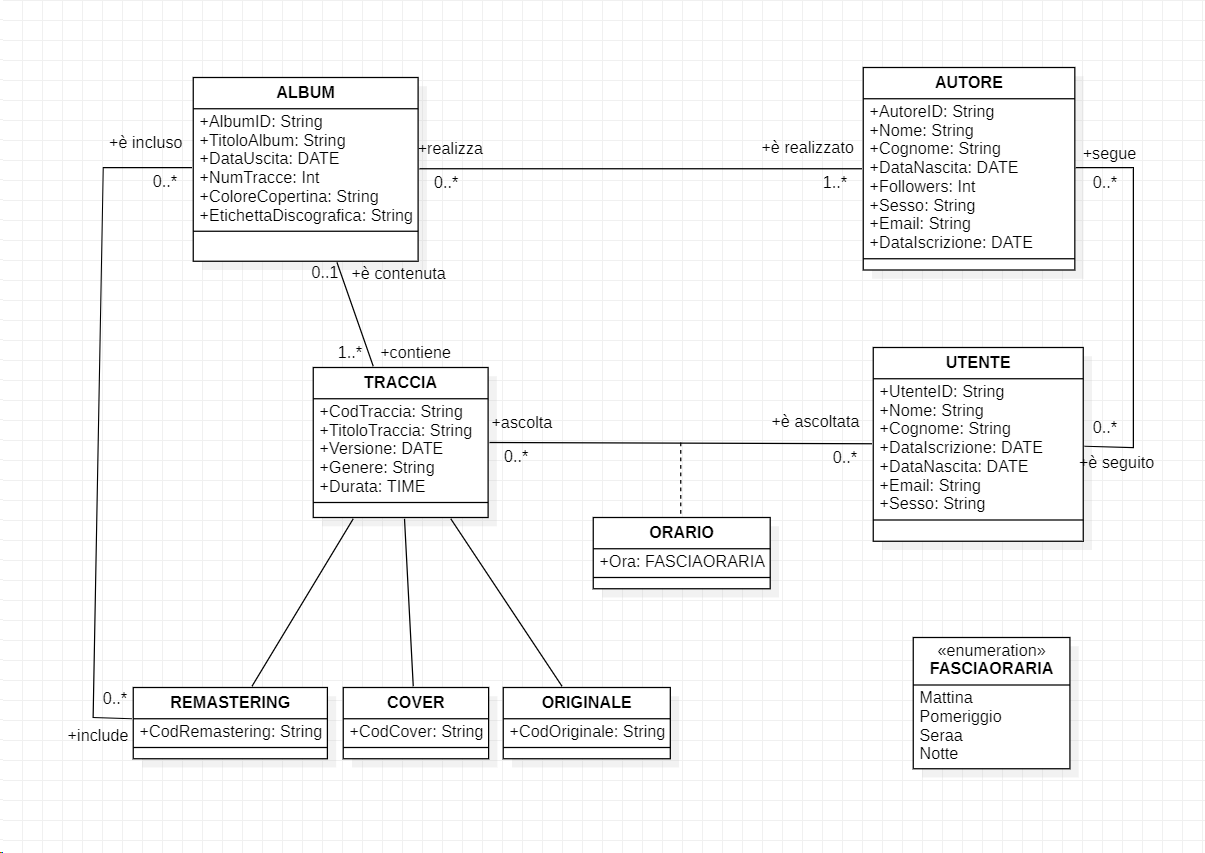
\includegraphics[scale = 0.5]{SpotifyPezzotto}
	\end{figure}

	\clearpage

	\begin{figure}
		\section{Class Diagram Ristrutturato}
		Per rendere il class diagram più vicino alla progettazione logica e alla realizzazione di 
		tabelle sul database, si è provveduto a ristrutturarlo.\\
		In particolare, come prima fase si è analizzato il contenuto delle classi per cercare 
		eventuali ridondanze.\\
		In una fase successiva sono state analizzate le associazioni, in particolare le gerarchie di specializzazione,
		sono state rese associazioni.\\
		\includegraphics[scale = 0.6]{SpotifyRistrotturato}

	\end{figure}

	In Particolare:\\
	\begin{description}
		
		\item[ELIMINAZIONE DELLA SPECIALIZZAZIONE]
		Una traccia può essere un 'Remastering', una cover, o un originale. 
		Eliminiamo la specializzazione e inseriamo all’interno della classe \textbf{TRACCIA} un attributo discriminante, 
		ossia \textbf{TIPOTRACCIA} che potrà avere valore uguale a 'Remastering','Live', 'Remix','Cover' oppure 'Originale'.
		Differenziamo il caso in cui \textbf{TIPOTRACCIA} avesse valore uguale a 'Cover', 'Remastering', 'Live', 'Remix';
		introduciamo l’attributo \textbf{CodTracciaOriginale"} per poter risalire alla traccia originale\\
		\item[ELIMINAZIONE DELLE RITONDANZE]
		Nel class diagram originale apparivano attributi che possono essere “calcolati” tramite una query, come NumTracce nella classe ALBUM e Followers di \textbf{UTENTE}.\\
		Inoltre, le classi \textbf{AUTORE} e \textbf{UTENTE} risultano essere costituite da attributi pressoché simili;
		fondiamo le due classi nella classe \textbf{UTENTE} e definiamo l’associazione following come ricorsiva.
		Per distinguere il caso di Autore e Ascoltatore abbiamo introdotto un nuovo attributo discriminante: \textbf{TIPOUTENTE}.
		Nella classe Utente è stato eliminato l’attributo Followers in quando tale informazione è recuperabile tramite la classe \textbf{FOLLOWERS}.\\
	\end{description}

	\clearpage

	\section{Dizionari}
	\subsection{Dizionario delle Classi}

	\begin{table}[h]
		\centering
		\begin{adjustbox}{max width=\textwidth}
			\begin{tabular}{|l|l|l|} \hline
			CLASSE  & DESCRIZIONE                                                                                                                                                                                        & ATTRIBUTI                                                                                                                                                                                                                                                                                                                                                                                                                                                                                                                                                                                                                                              \\\hline
			\hline
			ALBUM   & \begin{tabular}[c]{@{}l@{}}Descrittore del supporto \\ discografico, contenente \\ una racccolta di tracce\\ musicali di uno stesso autore/artista \\ o più autori/artisti differenti\end{tabular} & \begin{tabular}[c]{@{}l@{}}ALBUMID(integer): identificativo dell'album\\ TitoloAlbum(string): nome dell’album\\ N\_Tracce(Integer): numero di tracce contenuteDataUscita(Date): riferimento temporale dell’album \\ ColoreCopertina(String): colore scelto per la \\ copertina dell’album \\ EtichettaDiscografica(String): Marchio commerciale creato dalla casa discografica \\ che ha lavorato sull’album\end{tabular}                                                                                                                                                                                                                              \\\hline
			\hline
			TRACCIA & \begin{tabular}[c]{@{}l@{}}Unità che compone un album \\ discografico. E’ un brano musicale.\end{tabular}                                                                                          & \begin{tabular}[c]{@{}l@{}}TitoloTraccia(String): nome/titolo associato alla traccia che consente di scegliere cosa ascoltare.\\ Genere(String): genere musicale a cui appartiene la traccia \\ Durata(Time): tempo necessario per l’ascolto completo della traccia \\ TracciaID(integer): Identificatore univoco della traccia \\ Versione(date): anno della traccia originale se essa è una remastering\\ T\_Traccia(tipotraccia): ci da informazioni sulla tipologia \\ (cover,remastering,originale,live,remix) \\ CodTracciaOriginale(String):in caso di cover/remastering/live/remix ci da il riferimento \\ alla traccia originale\end{tabular} \\\hline
			\hline
			UTENTE  & \begin{tabular}[c]{@{}l@{}}Identità virtuale che usufruisce della \\ piattaforma musicale\end{tabular}                                                                                             & \begin{tabular}[c]{@{}l@{}}UtenteID (String): Identificativo univoco scelto dall’utente che comparirà al pubblico \\ sulla piattaforma \\ Nome(String): Nome ufficiale dell’utente \\ Cognome(String): Cognome ufficiale dell’utente \\ Email(String): email personale utilizzata dall’utente per accedere alla piattaforma \\ DataIscrizione(String): Data dell’iscrizione alla piattaforma\\ T\_Utente(TipoUtente) : Ci dice se l’utente è un autore o un ascoltatore\end{tabular}                                                                                                                                                                   \\\hline
			\hline
			ORA     & \begin{tabular}[c]{@{}l@{}}Ci fornisce un riferimento temporale\\ Fascia oraria in cui viene ascoltata \\ una traccia da un utente\end{tabular}                                                    & \begin{tabular}[c]{@{}l@{}}Ora(FasciaOrariaFASCIAORARIA): indica se una determinata traccia è stata \\ ascoltata da quel determinato utente di mattina,pomeriggio,sera o notte un momento\\ della giornata (mattina,pomeriggio,sera,notte).\end{tabular}                                                                                                                                                                                                                                                                                                                                                                                             \\ \hline
			\end{tabular}
		\end{adjustbox}
	\end{table}

	\subsection{Dizionario delle Associazioni}
	\begin{table}[h]
		\centering
		\begin{adjustbox}{max width=\textwidth}
			\begin{tabular}{|l|l|l|}
			\hline
			NOME          & DESCRIZIONE                                                                                                                                                          & CLASSI COINVOLTE                                                                                                                                                                                                                                                                                                              \\ \hline
			\hline
			REALIZZAZIONE & \begin{tabular}[c]{@{}l@{}}Esprime la relazione tra chi ha progettato/realizzato\\ l’album e l’album stesso\end{tabular}                                             & \begin{tabular}[c]{@{}l@{}}Autore{[}0…*{]} ruolo “realizza”: indica che l’autore può realizzare nessuno o molti album. \\ Album{[}1…*{]} ruolo “è realizzato”: indica che un album può essere creato da uno o più \\ autori\end{tabular}                                                                                      \\ \hline
			\hline
			SEGUITO       & \begin{tabular}[c]{@{}l@{}}Descrive la connessione tra gli autori e gli utenti della piattaformatra \\ gli utenti come autori e utenti come ascoltatori\end{tabular} & \begin{tabular}[c]{@{}l@{}}Autore{[}0…*{]} ruolo “è seguito”: indica che l’autore può essere seguito \\ da nessuno o da più utenti \\ Utente{[}0..*{]} ruolo “segue”: indica che l’utente può seguire \\ nessuno/più utenti\end{tabular}                                                                                      \\ \hline
			\hline
			ASCOLTO       & Ci da informazioni sul momento in cui un utente ascolta una traccia                                                                                                  & \begin{tabular}[c]{@{}l@{}}Utente{[}0…*{]} ruolo “ascolta”: indica che l’utente può ascoltare \\ nessuna o piu tracce Traccia{[}0…*{]}  ruolo “è ascoltata”\\ Orario{[}0…*{]} ruolo “è trascorsa”: indica che un momento della giornata può essere \\ utilizzato o meno da un utente sulla piattaforma\end{tabular}           \\ \hline
			\hline
			RIPRODUZIONE  & Ci da informazioni sul quando una traccia è ascoltata                                                                                                                & \begin{tabular}[c]{@{}l@{}}Traccia{[}0...*{]} ruolo “è riprodotta”: indica che una traccia può essere riprodotta o meno \\ in una fascia oraria.\\ Orario{[}0…*{]} ruolo “è utilizzata” : indica che un certo momento della giornata \\ può essere o meno utilizzato per ascoltare una traccia sulla piattaforma\end{tabular} \\ \hline
			\hline
			CONTIENE      & Descrive l’appartenenza di tracce negli album                                                                                                                        & \begin{tabular}[c]{@{}l@{}}Album {[}1…*{]} ruolo “contiene”: indica che un album contiene almeno una traccia. \\ Traccia{[}1…*{]} ruolo “è contenuta”: indica che una traccia deve essere contenuta in \\ almeno un album.\end{tabular}                                                                                       \\ \hline
			\hline
			\end{tabular}
		\end{adjustbox}
	\end{table}


	\clearpage
	\subsection{Dizionario dei Vincoli}
	\begin{table}[h]
		\centering
		\begin{adjustbox}{max width=\textwidth}
			\begin{tabular}{|l|l|}
				\hline
				NOME VINCOLO                  & DESCRIZIONE                                                                                                                                                                                                                                                              \\ \hline
				\hline
				CorrectEmailUtente                  & \begin{tabular}[c]{@{}l@{}}Gli indirizzi e-mail degli utenti devono essere indirizzi email di forma legittima, \\ ovvero contenere almeno un carattere prima della @, almeno un carattere tra essa \\ e il punto e almeno due caratteri nella parte finale.\end{tabular} \\ \hline
				\hline
				CorrectBirthUtente                  & La DataNascita di un utente deve essere precedente a DataIscrizione.                                                                                                                                                                                                     \\ \hline
				\hline
				UnicitàEmail                  & Una stessa email non può essere associata a utenti diversi.                                                                                                                                                                                                              \\ \hline
				\hline
				UnicitàUtenteID               & Uno stesso UtenteID non può corrispondere ad utenti diversi.                                                                                                                                                                                                             \\ \hline
				\hline
				UnicitàAlbumID                & Non possono esistere album diversi con AlbumID uguali.                                                                                                                                                                                                                   \\ \hline
				\hline
				UnicitàTracciaID              & Tracce diverse non possono avere TracciaID uguali.                                                                                                                                                                                                                       \\ \hline
				\hline
				LimitiDurataTraccia           & Durata deve avere un valore compreso tra 00:00:05 secondi e 01:00:00 ora .                                                                                                                                                                                                            \\ \hline
				\hline
				ParzialitàCodTracciaOriginale & \begin{tabular}[c]{@{}l@{}}L’attributo CodTracciaOriginale ha valore associato \\ solo se T\_Traccia è Remastering, Cover, Live, o Remix.\end{tabular}                                                                                                                   \\ \hline
				\hline
				VincoloTipologiaTraccia       & \begin{tabular}[c]{@{}l@{}}Una traccia con T\_Traccia di valore 'Remastering' \\ ha titolo e autore uguali ma deve avere versione e titoloAlbum diversi.\\ Le restanti tipologie di traccia non possono appartenere ad album diversi.\end{tabular}                         \\ \hline
				\hline
				VincoloRealizzazioneAlbumNotArtista          & L’associazione realizzazione è valida solo se T\_Utente è Autore.                                                                                                                                                                                                            \\ \hline
				\hline
				VincoloRealizzazioneAlbumUguali          & Lo stesso Autore non può publicare due Album con lo stesso nome                                                                                                                                                                                                            \\ \hline
			\end{tabular}
		\end{adjustbox}
	\end{table}

	\part{Progettazione Logica}
	\section{Schema logico}
	Di seguito, la rappresentazione della progettazione logica derivata dal class diagram
	revisionato e che va a costituire la struttura tabellare del database relazionale.
	Gli attributi sottolineati rappresentano le chiavi primarie, mentre quelli con doppia 
	sottolineatura indicano le chiavi esterne.\\
	\vspace{1cm}

	\begin{tabbing}
		\textbf{ASCOLTI} \= ( AscoltatoreID, TracciaID, ora ) \= \kill
		\textbf{UTENTE} \> ( \underline{UtenteID}, Nome, Cognome, DataNascita, DataIscrizione, Email, T\_Utente )\\\\
		\textbf{ALBUM} \> ( \underline{AlbumID}, TitoloAlbum, \underline{\underline{ArtistaID}}, ColoreCopertina, EtichettaDiscografica, DataUscita ) \\\\
		\textbf{TRACCIA} \> ( \underline{TracciaID}, \underline{\underline{AlbumID}}, TitoloTraccia, Durata, T\_Traccia, CodTracciaOriginale ) \\\\
		\textbf{SEGUITO} \> ( \underline{\underline{Segue}}, \underline{\underline{Seguito\_da}} )\\\\
		\textbf{ASCOLTI} \> ( \underline{\underline{AscoltatoreID}}, \underline{\underline{TracciaID}}, ora )
	\end{tabbing}
	
\end{document}